

\chapter{Discrete Systems}\label{chap:discrete_Model}
Contrary to continua, in discrete systems the motion of individual objects in the system and their interactions on each other is studied. In the following section, the mathematical formulations of such systems are described.
\section*{Definitions}
%For a reference on the notations used in the following sections, please see Chapter \ref{chap:nomenclature}.
Throughout section \S\ref{chap:discrete_Model}, the following conventions are used to denote the quantities associated with discrete systems. Scalar variables are denoted by uppercase or lowercase lightface Latin and Greek letters, e.g. $\rho$ and $\phi$. Vectors are denoted via bold, lowercase Latin letters, e.g. $\vect{x}$ and they are column vectors unless otherwise specified. More specifically, the variables $\vect{x}$, $\vect{v}$, $\vect{a}$ are used to represent the position, velocity and acceleration of an object. Indexed vectors are used to specify either an element of the vector or an object in the vector depending on the context, e.g. $\vect{x}_i$ is the position of body $i$. The first time-derivative is represented with over dot, e.g. $\dot{\vect{x}} = \vect{v}$.  The second time-derivative is denoted via over double-dot, e.g. $\ddot{\vect{x}} = \dot{\vect{v}} = \vect{a}$.  Matrices are represented as bold uppercase Latin letters, e.g. $\matr{M}$. One subscript is used to specify a single row, e.g. $\matr{M}_i$ for row $i$ in the matrix $\matr{M}$. Two subscripts are used to indicate a specific row and column, e.g. $\matr{M}_{i,j}$.   
The Frobenius norm of a matrix or a vector is defined as $\|*\|_F$. The skew-symmetric cross product operator for a three dimensional vector is defined as follows and results in a $3\times 3$ matrix
\begin{equation}
\tilde{{\vect s}} = \begin{bmatrix}
0 & -{s}_z & {s}_y\\ 
{s}_z & 0 & -{s}_x\\ 
-{s}_y & {s}_x & 0.
\end{bmatrix}
\end{equation}
\section{Rigid Body Dynamics}\label{sec:RigidBody}
In this section we describe the dynamic systems featuring rigid bodies and frictional contact between them. As explained in Section \S\ref{sec:back_rigid}, a complementarity-based approach is used to resolve the contact between different objects. 

\subsection*{Preamble}
``Rigid body'' refers to a 3D object that can translate and rotate in space. The set of generalized coordinates that describe the position and orientation of a body in the 3D Euclidean space are $\br_j\in \mathbb{R}^3$ and $\vect{\epsilon}_j\in \mathbb{R}^4$, which are respectively the absolute position of the center of mass, and Euler parameters associated with orientation of body $j$. Combining the set of generalized coordinates of different bodies for a system of $n_b$ bodies, one can write the set of generalized coordinates describing the system at position level as $\vect{x} = \left[ \vect{r}_1^T, \vect{\epsilon}_1^T,\ldots,\vect{r}_{n_b}^T, \vect{\epsilon}_{n_b}^T \right]^T \in \mathbb{R}^{7 n_b} $, and at velocity level as  $\dot{\vect{x}} = \left[ \dot{\vect{r}}_1^T, \dot{\vect{\epsilon}}_1^T,\ldots, \dot{\vect{r}}_{n_b}^T, 
\dot{\vect{\epsilon}}_{n_b}^T \right]^T$ $\in \mathbb{R}^{7 n_b}$. One can choose to use angular velocities instead of the time derivative of the Euler parameters to describe the system at the velocity level by  $\vect{v} = \left[ \dot{\vect{r}}_1^T, \bar{\vect{\omega}}_1^T,\ldots, \dot{\vect{r}}_{n_b}^T, 
\bar{\vect{\omega}}_{n_b}^T \right]^T$ $\in \mathbb{R}^{6 n_b}$, which reduces the problem size. The transformation from the derivatives of Euler parameters, ${\dot{\vect{\epsilon}}}_{B}$, to angular velocities at the body-fixed frame, ${\bar{\vect{\omega}}}_{B}$, for each body is governed by ${\dot{\vect{\epsilon}}}_{B}=\frac{1}{2} {\matr{G}}^T(\vect{\epsilon}_{B}) {\bar{\vect{\omega}}}_{B} $, where matrix ${\matr{G}}\in {\mathbb{R}}^{3 \times 4}$ depends linearly on the Euler parameters ${\vect{\epsilon}}_{B}$. Therefore, if one chooses to work with Euler angles at the velocity level, the block diagonal matrix  ${\vect L}(\vect{q}) \equiv \mbox{diag} \left[{{\matr I}}_{3 \times 3}, \frac{1}{2} {\matr{G}}^T(\vect{\epsilon}_{1}),\ldots,{\matr I}_{3 \times 3}, \frac{1}{2} {\matr{G}}^T(\vect{\epsilon}_{n_b})\right] \in {\mathbb{R}}^{7 n_b \times 6 n_b}$ can be used to obtain ${\dot{\vect{x}}} = {\vect L}({\vect{q}}) \vect{v}$, the time derivative of the set of generalized coordinate describing the system, where ${\matr I}_{3 \times 3}$ is the identity matrix \cite{Haug89}. 
\subsection{Bilateral Constraints}
A bilateral constraint represents a kinematic relationship between generalized coordinates in a discrete system. Spherical joints, prismatic joints, or revolute joints are examples of mechanical constraints that are comprised of a set of bilateral constraints represented by  $\mathcal{B}$. Hence, $\vect{g}_i\left(\vect{q},t\right)=\vect{0},i\in \mathcal{B}$ is a set of scalar equations to enforce kinematic constraints through algebraic equality equations. For instance, a revolute joint imposes five constraint equations, while a spherical is comprised of three constraint equations \cite{Haug89}.

The velocity-level constraint equations which must be satisfied are obtained by taking time-derivative of the constraints as  $\nabla_q \vect{g}_i^T \matr{L}\left(\vect{q}\right)\vect{v}+\dfrac{\partial\vect{g}_i}{\partial t}=0$.

\subsection{Unilateral Constraints and Frictional Contact}\label{sec:DVI}
In the Differential Variational Inequality (DVI) \cite{pastew03dvi} approach the equations of motion are modified to include a differential inclusion \cite{filippov1967classical} and to impose non-penetration between rigid bodies through constraints enforced by applying impulses. After discretization this problem is posed as an optimization problem with complementarity and equilibrium constraints. More specifically, the three-dimensional Coulomb friction assumption leads to a Non-linear Complementarity Problem (NCP).  In what follows, more details about the theory of the complementarity approach are explained.

Consider a contact between bodies $A$ and $B$ as shown in Fig.~\ref{fig:DVI_Contact}. The tangent plane at the contact point for the contact $i$ is defined by vectors $\textbf{u}_i$, $\textbf{w}_i$ and the normal $\textbf{n}_i$ in Fig.~\ref{fig:DVI_Contact}. A local reference frame can be defined for each body at the contact point based on these vectors. For body $A$, the normal to the tangent plane, $\textbf{n}_{i,A}$, points toward body $B$. The two mutually orthogonal vectors $\textbf{u}_{i,A}$, and $\textbf{w}_{i,A}$ are defined using the Gram-Schmidt method. The same methodology is used to build the local reference frame at the contact point $i$, for body $B$ with $\textbf{w}_{i,B}$, $\textbf{u}_{i,B}$, and $\textbf{n}_{i,B}$ $\in \mathbb{R}^3$. 

\begin{figure}
	\begin{center}
		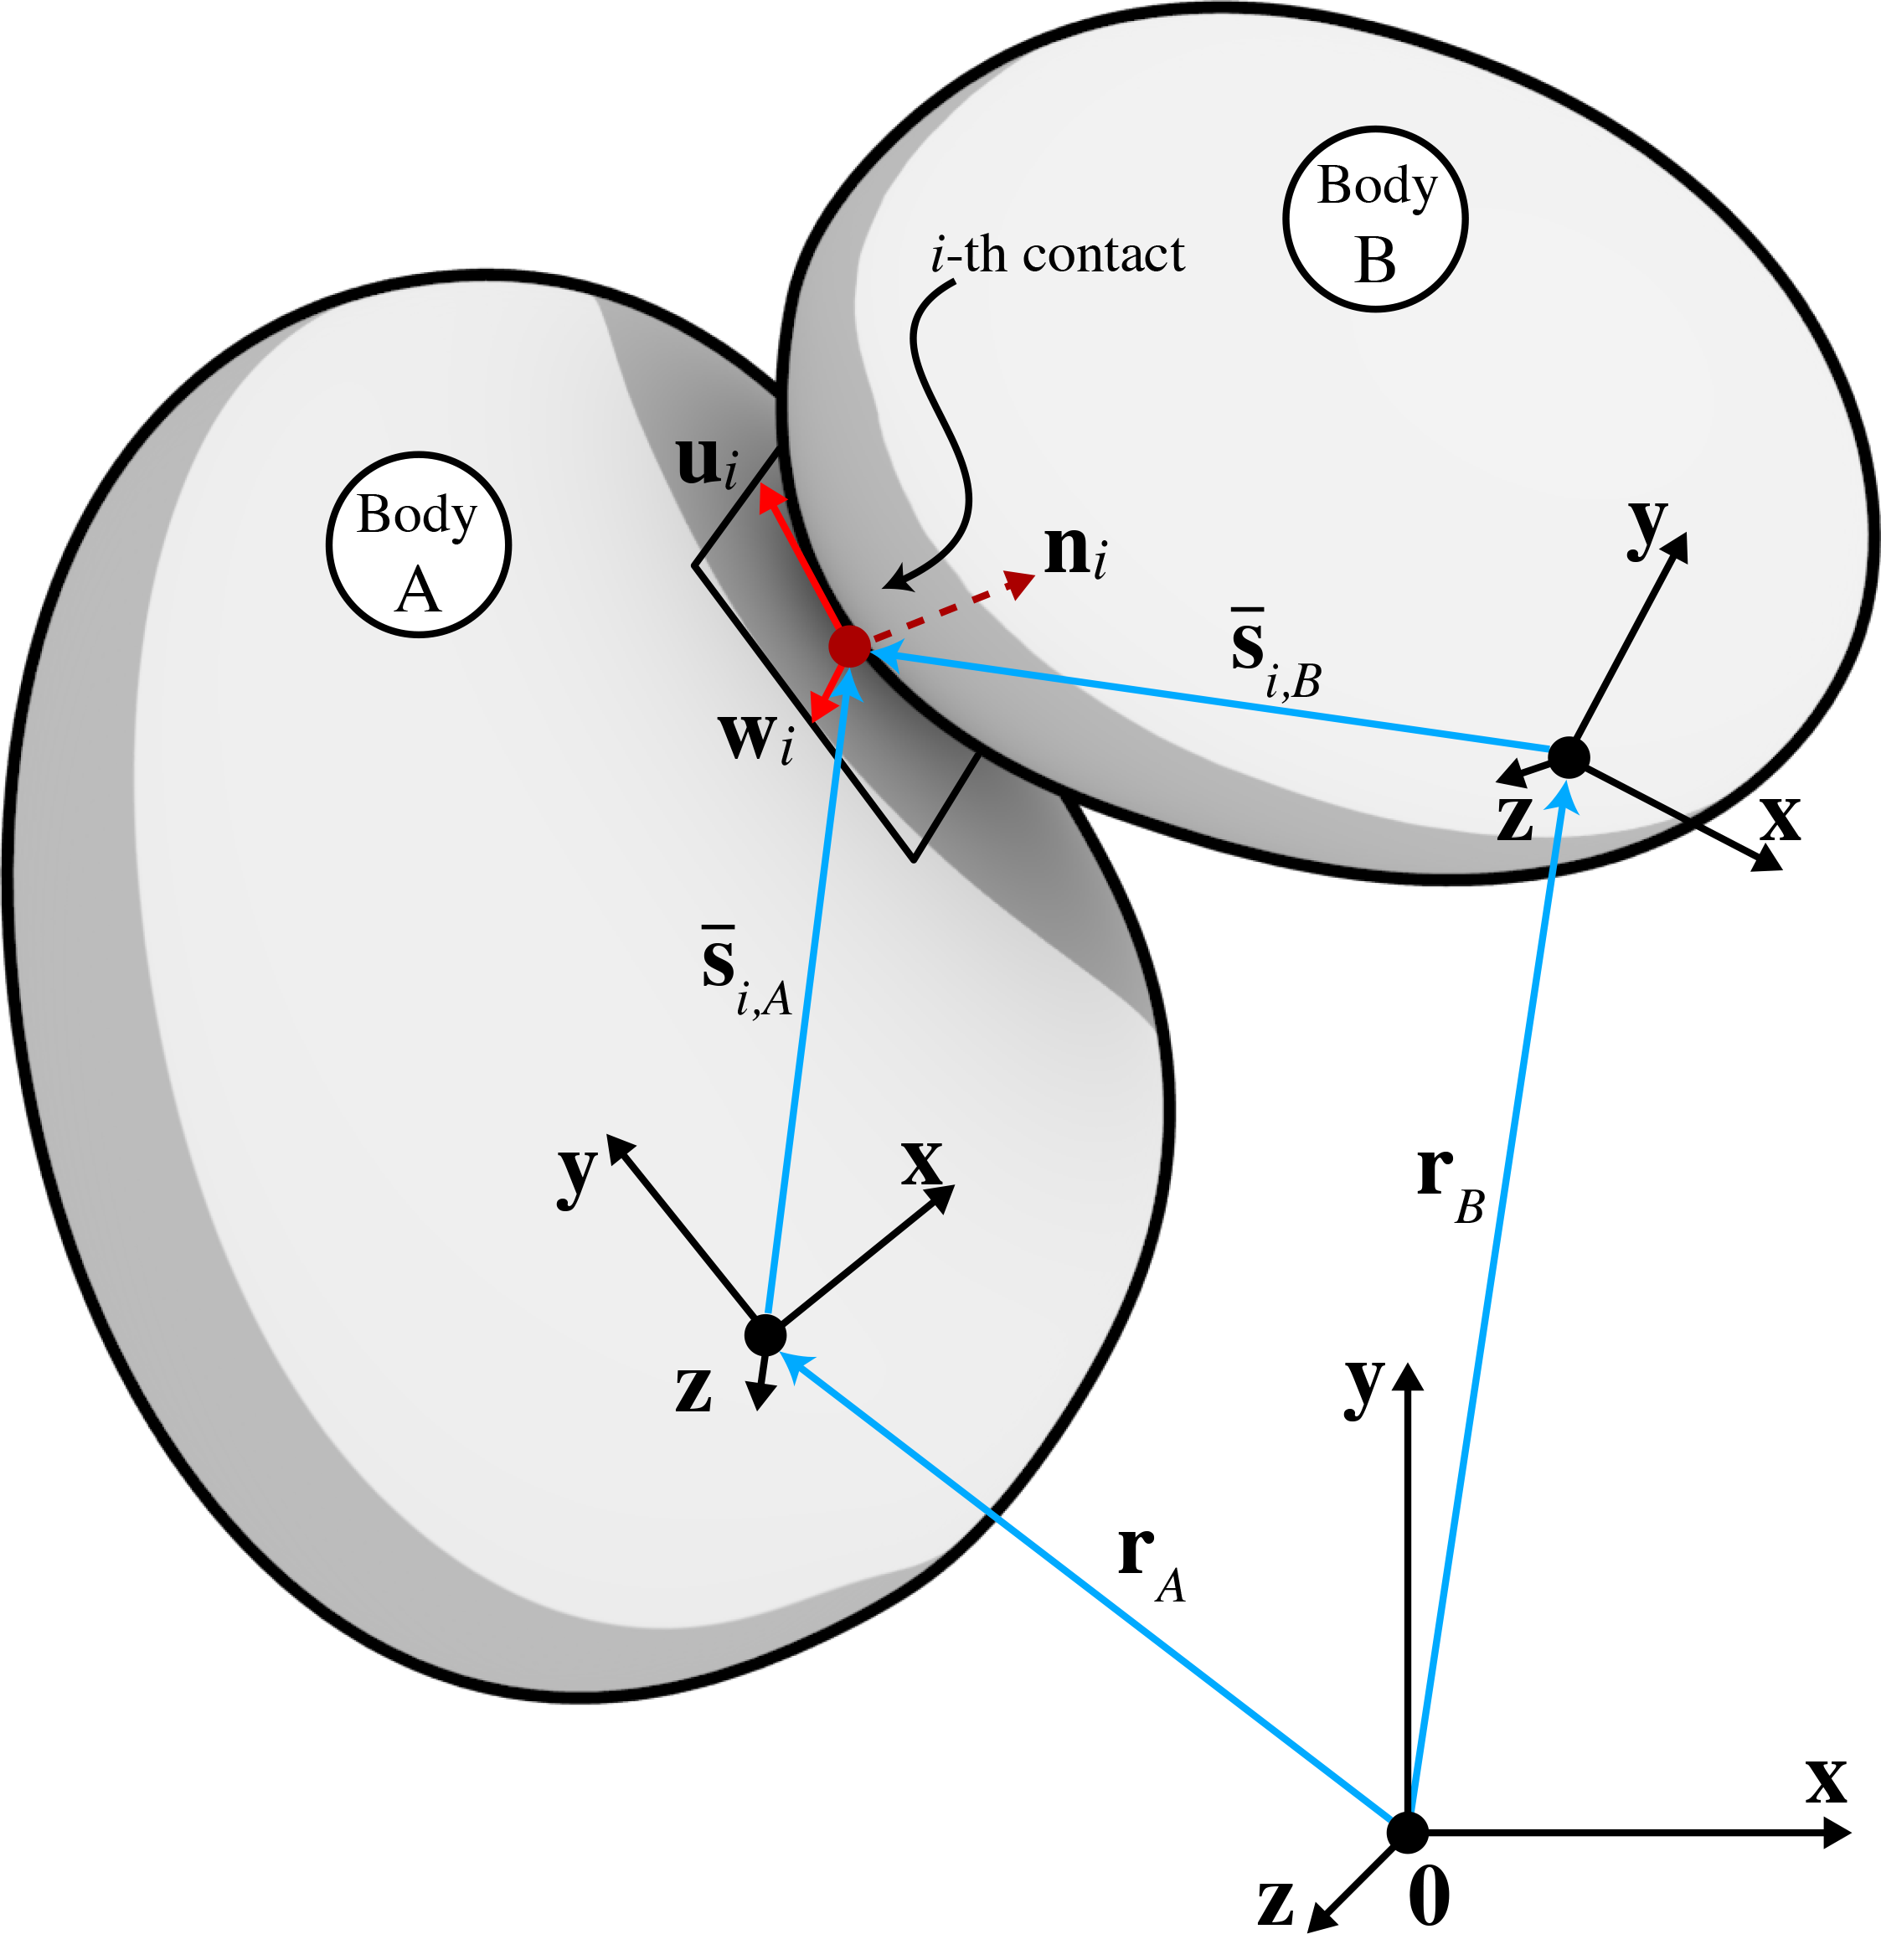
\includegraphics[width=.4\linewidth]{images/twobodies.png}
	\end{center}
	\caption{Schematic of contact between two bodies.}
	\label{fig:DVI_Contact}
\end{figure}

If the gap (distance) between bodies $A$ and $B$ at the contact point is defined by $\Phi$, a complementarity condition can be defined as $0 \leq \widehat{\gamma}^c_{i,n}  \perp \Phi \geq 0$, where $\widehat{\gamma}^c_{i,n}$  is the Lagrange multiplier associated with the contact $i$. The complementarity condition states that at least one of the $\widehat{\gamma}^c_{i,n}$, or $\Phi$ is zero; when the gap function is zero, the normal contact force is greater than zero and when the normal contact force is zero the gap function is greater than zero (there is no contact between body $A$ and $B$). The contact force associated with contact $i$ can be expressed as $\vect{f}_{i,N}=\widehat{\gamma}^c_{i,n}\vect{n}_i$, and $\vect{f}_{i,T}=\widehat{\gamma}^c_{i,u}\vect{u}_i+\widehat{\gamma}^c_{i,w}\vect{w}_i$ which are the normal and tangential forces, respectively.  $\widehat{\gamma}^c_{i,w}$, $\widehat{\gamma}^c_{i,u}$, and $\widehat{\gamma}^c_{i,n}$ are the magnitude of the contact forces in each direction. The Coulomb dry-friction model based on the friction forces is expressed as  \cite{StTr95,stewartSIAMreview2000}
\begin{subequations}
	\begin{align}
	\label{eq:FrictionModel_1}
	\sqrt{(\widehat{\gamma}^c_{i,u})^2+(\widehat{\gamma}^c_{i,w})^2}\leq \mu^f_{i} \widehat{\gamma}^c_{i,n}&,\\ 
	\label{eq:FrictionModel_2}
	\quad \lVert\vect{v}_{i,T}\rVert\left(\sqrt{(\widehat{\gamma}^c_{i,u})^2+(\widehat{\gamma}^c_{i,w})^2} - \mu^f_{i} \widehat{\gamma}^c_{i,n} \right)=0&,\\
	\label{eq:FrictionModel_3}
	\langle\vect{f}_{i,T},\vect{v}_{i,T}\rangle=-\lVert\vect{f}_{i,T}\rVert\lVert\vect{v}_{i,T}\rVert \;&,
	\end{align}
\end{subequations}
where $\vect{v}_{i,T}$ denotes the relative tangential velocity between bodies $A$ and $B$ at the contact point. More specifically, Eq.~\ref{eq:FrictionModel_1} states that the the friction force is less than the normal force times the friction coefficient.  Eq.~\ref{eq:FrictionModel_2} states a complementarity condition where equality condition of Eq.~\ref{eq:FrictionModel_1} holds if the $\vect{v}_{i,T}\not=0$, and inequality of Eq.~\ref{eq:FrictionModel_1} holds if $\vect{v}_{i,T}=0$. Lastly, Eq.~\ref{eq:FrictionModel_3} states that the friction force is in the opposite direction of $\vect{v}_{i,T}$. If now one considers the following constraint minimization problem, 
\begin{equation}
\label{eq:fricMin}
\left( \widehat{\gamma}^c_{i,u},\widehat{\gamma}^c_{i,w} \right) = \mathop {\mbox{argmin}}\limits_{\sqrt{(\widehat{\gamma}^c_{i,u})^2+(\widehat{\gamma}^c_{i,w})^2} \leq \mu^f_{i} \widehat{\gamma}^c_{i,n}}
{\mathbf v}_{i,T}^T \left( \widehat{\gamma}^c_{i,u} \uVec{i} + \widehat{\gamma}^c_{i,w} \wVec{i} \right),
\end{equation}
then Eq.~\ref{eq:FrictionModel_1}-\ref{eq:FrictionModel_3} represent the first order Karush-Kuhn-Tucker optimality condition for the above optimization problem with respect to $\widehat{\gamma}^c_{i,u}$, and $\widehat{\gamma}^c_{i,w}$ variables. Hence, the Coulomb friction model is implemented as a constraint optimization problem. Finally, the contact force at the $i^{th}$ contact point is expressed as $\vect{f}_i=\vect{f}_{i,N}+\vect{f}_{i,T}=\widehat{\gamma}^c_{i,n}\vect{n}_i+\widehat{\gamma}^c_{i,w}\vect{u}_i+\widehat{\gamma}^c_{i,w}\vect{w}_i \in \cone_i$,  where $\cone_i$ is a 3D cone of slope $\tan^{-1}(\mu^f_{i})$ and oriented along $\vect{n}_i$, i.e., $\cone_i=\{\left[x,y,z\right]^T \in \mathbb{R}^3 | \sqrt{y^2+z^2} \leq \mu^f_{i} x\}$.


The Newton-Euler equations of motion for the system \cite{StTr95} are expressed as:
\begin{equation}
\label{eq:Newton_Euler}
\begin{gathered}
\begin{array}{rcl}
{\mathbf{\dot q}}   & = &  {\bf L}({\mathbf{q}}){\bf v} \vspace{0.2cm},  \\ 
{\mathbf{M}} {\mathbf{\dot v}} & = &{\mathbf{f}}\left( {t,  {\bf q} , {\bf v} } \right) -\vect{g}_{\vect{q}}^T\left(\vect{q},t\right)\lambda  + \vspace{0.2cm} \sum\limits_{i\in \cA({\bf q},\delta)} \left( \hatGN{i} \Pn{i} + \hatGU{i} \Ptu{i}  + \hatGW{i} \Ptw{i}  \right) \vspace{0.2cm}, \\
0 & = & {\bf g}({\bf q},t)\vspace{0.2cm}, \\ 
i \in \cA({\bf q}(t),\delta)  &:&  0 \le \hatGN{i} \; \perp \; \Phi_{i}({\bf q}) \geq 0 \vspace{0.2cm}, \\
\left(\hatGU{i}, \hatGW{i} \right)  &=&  \mathop {\mbox{argmin}}\limits_{\sqrt{(\widehat{\gamma}^c_{i,u})^2+(\widehat{\gamma}^c_{i,w})^2} \leq \mu^f_{i} \widehat{\gamma}^c_{i,n}} {\bf v}^T \left( \widehat{\gamma}^c_{i,u} \Ptu{i} + \widehat{\gamma}^c_{i,w} \Ptw{i} \right) \;,
\end{array}
\end{gathered} 
\end{equation}
where  $\mathbf{f}(t,  {\bf q} , {\bf v} ) $ are the external forces, $\textbf{M}$ is the system mass Matrix, $\cA({\bf q},\delta)$  is the set of active and potential unilateral constraints based on the bodies that are mutually less than $\delta$ apart, and $\textbf{g}(\textbf{q},t)$ is the set of bilateral constraints acting on the system and $\vect{g}_{\vect{q}}^T\left(\vect{q},t\right)$ is the Jacobian of the constraints with respect to the generalized coordinates. Moreover, the tangent space generators 
$\Proj{i}=[\Pn{i}, \Ptu{i}, \Ptw{i} ] \in {\mathbbm{R}}^{6n_b \times 3}$ are defined as
%
\begin{equation}
\begin{gathered}
\Proj{i}^{T} =
\left[ 
{\bf 0} \;\; \ldots \;\; - {\bf A}_{i,p}^T \;\; { {\bf A}_{i,p}^T {\bf{A}}_A {\tilde {\bar {\bf{s}}}}_{i,A}}  
\;\; {\bf 0} \;\;  \ldots  \;\;  {\bf 0} \;\;
{\bf A}_{i,p}^T \;\; { - {\bf A}_{i,p}^T {\bf{A}}_B  {\tilde {\bar {\bf{s}}}}_{i,B}  }  \;\; \ldots \;\;{\bf 0}
\right] ,
\end{gathered} 
\end{equation}
%
where ${\bf{A}}_{i,p} = [\nVec{i}, \uVec{i}, \wVec{i} ] \in {\mathbbm{R}}^{3 \times 3}$ is the orientation matrix associated with contact $i$,
${\bf{A}}_A={\bf{A}}\left({\bf \epsilon}_A\right)$ and ${\bf{A}}_B={\bf{A}}\left({\bf \epsilon}_B\right)$ are the rotation matrices of bodies $A$ and $B$ respectively; the vectors ${\bar {\bf s}}_{i,A}$ and ${\bar {\bf s}}_{i,B} \in {\mathbbm{R}}^{3}$  represent the contact point positions in body-relative coordinates as shown in Fig.~\ref{fig:DVI_Contact}. More details about the solution algorithm, and time-stepping scheme of the this DVI problem may be found in \cite{StTr95,ani04,aniha03}.


\subsection{Time Integration}
In the following, the superscript $(n)$ is used to represent values at time-step $t^{(n)}$, e.g.,  $\vect{q}^{(n)}$ and $\vect{v}^{(n)}$ represent the position and velocity at time-step $t^{(n)}$ respectively.
$\vect{\gamma}_i=h\hat{\vect{\gamma}}_i$ denotes contact impulse for contact $i$. The time integrated equations of motion discussed in Eq.~\ref{eq:Newton_Euler} for a time step $h$ is as follows:
\begin{align}
\vect{q}^{(l+1)}=&\vect{q}^{(l)}+h \matr{L}\left(\vect{q}^{(l)}\right)\vect{v}^{(l+1)} \label{eq:DVI_EOM_DISC:1},\\
\matr{M}\left(\vect{v}^{(l+1)}-\vect{v}^{(l)}\right)=&h \vect{f}\left(t^{(l)},\vect{q}^{(l)},\vect{v}^{(l)}\right)-\vect{g}_{\vect{q}}^T\left(\vect{q}^{(l)},t\right)\lambda, \nonumber \\
+&\sum\limits_{i=1}^{N_c} \left( \vect{\gamma}_{i,n} \matr{D}_{i,n}^T + \vect{\gamma}_{i,u} \matr{D}_{i,u}^T + \vect{\gamma}_{i,w} \matr{D}_{i,w}^T \right),\label{eq:DVI_EOM_DISC:2}\\
\underbrace{\frac{1}{h}\vect{g}\left(\vect{q}^{(l)},t\right)}_{\text{stabilization term}}+&\vect{g}_{\vect{q}}^T\matr{L}\left(\vect{q}^{(l)}\right)\vect{v}^{(l+1)}+\vect{g}_t=\vect{0} \label{eq:DVI_EOM_DISC:3},\\
\text{for} \quad i=1,2,\ldots,N_c, \nonumber\\
0 \leq \underbrace{\frac{1}{h}\Phi_i\left(\vect{q}^{(l)},t\right)}_{\text{stabilization term}}+&\matr{D}_{i,n}^T\vect{v}^{(l+1)}  \underbrace{-\mu_i \sqrt{\left(\matr{D}_{i,u}^T\vect{v}^{(l+1)}\right)^2+\left(\matr{D}_{i,w}^T\vect{v}^{(l+1)}\right)^2} }_{\text{relaxation term}}\perp \vect{\gamma}_{i,n} \geq 0, \label{eq:DVI_EOM_DISC:4}\\
\left(\vect{\gamma}_{i,u},\vect{\gamma}_{i,w}\right)=&\argmin_{\sqrt{\vect{\gamma}_{i,u}^2+\vect{\gamma}_{i,w}^2}\leq \mu_i\vect{\gamma}_{i,n}} \left(\vect{\gamma}_{i,u}{\vect{v}^{(l+1)}}^T \matr{D}_{i,u}+\vect{\gamma}_{i,w} {\vect{v}^{(l+1)}}^T \matr{D}_{i,w}\right) \label{eq:DVI_EOM_DISC:5}.
\end{align}
Above, the position level update Eq.~\ref{eq:DVI_EOM_DISC:1} follows the forward Euler scheme. Eq.~\ref{eq:DVI_EOM_DISC:2} is the time-discretized momentum balance featuring the reaction forces associated with bilateral (mechanical) and unilateral (contact) constraints.  Eq.~\ref{eq:DVI_EOM_DISC:3} is time-discretized algebraic equation for bilateral constraints. Eq.~\ref{eq:DVI_EOM_DISC:4} is the time-discretized scalar complementarity condition in the normal direction while Eq.~\ref{eq:DVI_EOM_DISC:5} is the minimization problem corresponding to the Coulomb friction model for frictional forces. Inclusion of the relaxation term in Eq.~\ref{eq:DVI_EOM_DISC:4} leads to a Cone Complementarity Problem (CCP), which represents the first order optimality condition of a Quadratic Optimization with Conic Constraints (QOCC). It has been shown in \cite{ani04} that the solution of the modified scheme will approach the solution of the original problem as the step-size goes to zero.
The underlying CCP is as follows:
\begin{align}\label{eq:DVI_CCP}
&\text{Find } \vect{\gamma}_i, \text{ for } i=1,\ldots,N_c \nonumber, \\
&\text{such that } {\mathcal{K}}_i \ni \vect{\gamma}_i\perp -\left(\matr{N}\vect{\gamma}+\vect{r}\right)_i \in {\mathcal{K}}_i^\circ ,\\
&\text{where}\; {\mathcal{K}}_i=\{\left[x,y,z\right]^T \in \mathbb{R}^3 | \sqrt{y^2+z^2} \leq \mu_i x\} \nonumber,\\
&\text{and}\; {\mathcal{K}}_i^\circ=\{\left[x,y,z\right]^T \in \mathbb{R}^3 | x \leq -\mu_i\sqrt{y^2+z^2}\}, \nonumber
\end{align}
where the superscript $^{(l+1)}$ in $\vect{\gamma}_i=\vect{\gamma}_i^{(l+1)}$ was omitted for clarity. The system level coefficient Matrix $\matr{N}$ and the vector $\vect{r}$ are defined as:
\begin{eqnarray}
\matr{N}&=&\matr{D}^T\matr{M}^{-1}\matr{D}, \\
\matr{r}&=&\vect{b}+\matr{D}^T\matr{M}^{-1}\vect{k}.
\end{eqnarray}
Above,  $\vect{b}_i = \left[\frac{1}{h}\Phi_i,0,0\right]^T$ for contact $i$, and $\vect{k}=\matr{M}\vect{v}^{(l)}+h \vect{f}\left(t^{(l)},\vect{q}^{(l)},\vect{v}^{(l)}\right)$.

\noindent
The equivalent QOCC of the above problem is as follows:
\begin{eqnarray}\label{eq:DVI_QOCC}
&&\min f\left(\vect{\gamma}\right) = \frac{1}{2}\vect{\gamma}^T \matr{N} \vect{\gamma}+\vect{r}^T \vect{\gamma} \label{eq:OPT_friction},\\
&&\text{subject to } \vect{\gamma}_i \in {\mathcal{K}}_i \text{ for } i=1,2,\ldots,N_c, \nonumber
\end{eqnarray}
\noindent
where $\vect{\gamma}_i$ is the triplet of multipliers associated with contact $i$ and $\vect{\gamma}_i\in{\mathcal{K}}_i$  as stated in Eq.~\ref{eq:DVI_CCP}.
Herein,  $\vect{\gamma}=\left[\vect{\gamma}_1^T,\vect{\gamma}_2^T,\ldots,\vect{\gamma}_{N_c}^T\right]^T$ is the system level vector of Lagrange multipliers (contact impulses) associated with unilateral constraints. The equivalence of Eqs.~\ref{eq:DVI_CCP} and \ref{eq:OPT_friction} has been verified by considering the KKT first-order necessary conditions in \cite{heynPhDThesis2013}. Various methods exist for solving Eqs.~\ref{eq:DVI_CCP} and \ref{eq:OPT_friction}. In \cite{heynPhDThesis2013} advantages and shortcomings of solution algorithms such as Jacobi, Gauss-Siedel, Accelerated Projected Gradient Descent (APGD), and interior-point method for solution of the problem in its optimization form, Eq.\ref{eq:OPT_friction}, were discussed.

\subsection{Solution Uniqueness}\label{sec:Uniqueness}
The complementarity method discussed in Eqs.~\ref{eq:DVI_CCP} or \ref{eq:DVI_QOCC} for idealized perfectly-rigid bodies does not have a unique solution. Specifically, this is due to the indeterminacy of the curvature matrix $\matr{N}$, which is typically positive semidefinite. A positive semidefinite matrix $\matr{N}$ emerges when there are many contacts per body. Thus, the system has infinitely many sets of reaction forces that satisfy the DVI equations. This non-uniqueness appears only in the normal forces for frictionless problems, while both the velocities and the contact forces are non-unique for frictional problems. Use of additional compatibility conditions for contact forces in frictionless problems was investigated in \cite{olsen2018resolving}. The compatibility condition maintains no-penetration constraints but filters out force distributions that could not have arisen from stiff elastic contacts. In the present work, we use the Tikhonov regularization method to improve the solution quality in frictional problems. 
Herein, the set of solution to Eq.~\ref{eq:DVI_QOCC} is denoted by 
\begin{equation}
\mathcal{S} = \{ \vect{\gamma} \in {\mathcal{K}}  \;| \; f(\vect{\gamma}) = \inf_{\vect{y} \in \mathcal{K}} \; f(\vect{y}) \}, 
\end{equation}
where $\mathcal{K}=\mathcal{K}_1\times\mathcal{K}_2 \hdots \times \mathcal{K}_{N_c}$  is the direct product of the individual contact cones.

The Tikhonov regularized QOCC of Eq.~\ref{eq:DVI_QOCC}  is modified as:
\begin{eqnarray}\label{eq:DVI_QOCC_reg}
&&\min f_\alpha \left(\vect{\gamma}\right) = \frac{1}{2}\vect{\gamma}^T \matr{N} \vect{\gamma}+\vect{r}^T \vect{\gamma} + \alpha \|\vect{\gamma}\|^2_W  \label{eq:OPT_friction_ref},\\
&&\text{subject to } \vect{\gamma}_i \in {\mathcal{K}}_i \text{ for } i=1,2,\ldots,N_c. \nonumber
\end{eqnarray}
The inclusion of the regularization term $\alpha \|\vect{\gamma}\|^2_W$ increases the zero eigenvalues of the $\matr{N}$ to ensure a unique solution. Note that the cost function in Eq.~\ref{eq:DVI_QOCC_reg} is strictly convex for ${\alpha}>0$. 

According to the Tikhonov regularization method, the minimum-norm solution of a \textit{convex} optimization problem may be obtained by solving a sequence of related \textit{strongly convex} optimization problems. Accordingly, the sequence ${\vect{\gamma}_k}$ generated by the Tikhonov regularized problem
\begin{equation}
 \vect{\gamma}^{k+1} = \underset{\vect{\gamma} \in {\mathcal{K}} }{\mathrm{argmin}} \{\frac{1}{2}\vect{\gamma}^T \matr{N} \vect{\gamma}+\vect{r}^T \vect{\gamma} + \alpha_k \|\vect{\gamma}\|^2_W   \},
\end{equation}
 converges to the minimum norm of $S$ as $\alpha \to 0^+$, which is sufficient from the theoretical perspective. However, one may choose not to find the exact solution of each subproblem, but solving it withing some tolerance $\epsilon_k$, in order to make the solution procedure more efficient. The idea is to solve the subproblem with looser tolerances at the beginning and with more strict tolerances as $\alpha \to 0^+$. In practice, one may choose to reduce the tolerance and the regularization parameter as $\epsilon_{k+1}=\tau_{\epsilon} \epsilon_{k}$ and $\alpha_{k+1}=\tau_{\alpha} \alpha_{k}$, for some constants $\tau_{\alpha}$ and $\tau_{\epsilon}$, where $0<\tau_{\epsilon}<\tau_{\alpha}<1$. 
 
 Alternatively, one may choose a small value of the regularization parameter $\alpha_k$ and solve only one subproblem and since the feasible set is convex for $\alpha>0$. This regularized problem has a unique solution although the solution may slightly differ from the classical Tikhonov regularization method described above. These ideas are investigated for a few benchmark problems in section \S\ref{sec:DVI_Uniq}.

\section{Flexible Body Dynamics}\label{sec:FMBD}
The nonlinear flexible body dynamics formulation used in the current work draws on ANCF, a nonlinear finite element formulation introduced by Shabana~\cite{Shabana1997} to describe large deformation of moving bodies. The salient feature of ANCF is the use of position vector gradients to describe the rotation of the body. ANCF uses the nodal global-position and the nodal position-vector-gradients to describe the nonlinear dynamics of flexible bodies that can undergo large deformation.
In general, the position field of $i^{th}$ ANCF element may be defined as: 
\begin{equation} \label{eq:ANCF_r}
\underbrace{{{\bm{r}}^{i}}(\xi,\eta,\zeta,t)}_{\begin{smallmatrix}
	\text{Position of an arbitrary } \\
	\text{point within the element}
	\end{smallmatrix}}=\underbrace{\bm{S}(\xi,\eta,\zeta)}_{\begin{smallmatrix}
	\text{Space-dependent } \\
	\text{shape function}
	\end{smallmatrix}}\times \underbrace{{{\bm{q}}^{i}}(t),}_{\begin{smallmatrix}
	\text{Time-dependent vector of } \\
	\text{nodal degrees of freedom}
	\end{smallmatrix}}
\end{equation}
which simply gives the position of any point $(\xi,\eta,\zeta) \in [-1,1]$ inside the element at time $t$ based on interpolation ($\bm{S} (\xi,\eta,\zeta) $) of the nodal coordinates ($\bm{q}^{i}(t)$). Due to the fact that description of elements is in global coordinates, the inertia forces have a simple form in ANCF elements. The velocity of any point within an element $i$ may be written as
\begin{equation} \label{eq:ANCF_r_dot}
\underbrace{\bm{\dot{r}}^{i}(\xi,\eta,\zeta,t)}_{\begin{smallmatrix}
	\text{Velocity of an arbitrary } \\
	\text{point within the element}
	\end{smallmatrix}}=\underbrace{\bm{S}(\xi,\eta,\zeta)}_{\begin{smallmatrix}
	\text{Space-dependent } \\
	\text{shape function}
	\end{smallmatrix}}\times \underbrace{\bm{\dot{q}}^{i}(t).}_{\begin{smallmatrix}
	\text{Time-dependent vector of } \\
	\text{generalized velocities}
	\end{smallmatrix}}
\end{equation}
The kinetic energy of a finite element $i$ can be obtained as
\begin{equation} \label{eq:ANCF_T}
T = \frac{1}{2}\int\limits_V {\rho {{{\mathbf{\dot r}}}^{i\text{T}}}{\mathbf{\dot r}}^{i}} {\text{ d}}V = \frac{1}{2}{{\mathbf{\dot q}}^{i\text{T}}}{\mathbf{M\dot q}^{i}}\;,
\end{equation}
where the mass matrix ${\mathbf{M}}$ is defined as \small ${\mathbf{M}} = \int_A {\rho A {{\bm{S}}^\text{T}}{\bm{S}}} {\text{ d}}x$, which is time-independent. The equations of motion assume the form \cite{shabana2013} 
\begin{equation}
\mathbf{M} \ddot{\mathbf{q}} + \mathbf{{Q}}_e=\mathbf{{Q}}_a\;,
\end{equation}
where  $\mathbf{{Q}}_e$ and $\mathbf{{Q}}_a$ are the generalized element elastic and applied forces, respectively. The description of these elements and calculation of the internal forces are described in \S \ref{sec:1DElem}, and \S \ref{sec:2DElem}.

ANCF elements may be classified based on the number of position vector gradients defined at each node. ($i$) \textbf{Fully parameterized} ANCF elements use position vector $r \in \mathbb R^3$, and 3 position vector gradients, $\bm{r}_x$, $\bm{r}_y$, and $ \bm{r}_z  \in \mathbb R^3 $ where $x$, $y$, and $z$ are the natural coordinates of the element. Fully parameterized elements allow for easy implementation of the continuum mechanics approach to calculate the deformation gradient ($\textbf{F}$). ($ii$) \textbf{Gradient Deficient} ANCF elements use position vector $r \in \mathbb R^3$, and fewer than 3 position vector gradients, when using fewer position vector gradients is sufficient to define the volume used in continuum mechanics approach. Using fewer position gradient vectors has been shown to eliminate various locking problems.

Development of ANCF elements is still an ongoing research topic, yet in the current work elements that have been shown robust and acceptable accuracy are chosen for the simulations of the flexible bodies. More specifically, ANCF cable element, ANCF shell element, and hexahedron brick elements, which are appropriate respectively for modeling 1D, 2D, and 3D bodies, are to be used in the FE analysis of this present work.


\subsection{ANCF Cable Element}\label{sec:1DElem}
The gradient-deficient ANCF cable element introduced by Berzeri and Shabana~\cite{berzeri2000} is used in the present work. As shown in Fig.~\ref{fig:ANCFCable}, the coordinates of this element at each node are a position vector and a position vector gradient along the beam central axis. The position gradient vectors normal to the cable axis are not defined, hence the element is gradient deficient. Subsequently, torsion and shear deformation cannot be captured with this set of degrees of freedom. The coordinates (nodal degree of freedom) of the $j^{th}$ node is expressed as the $6 \times 1$ matrix \small${{\bm{q}}^{j}}(t)={{\left[ \begin{matrix}
		\bm{r}_{{}}^{j\text{T}} & \bm{r}_{x}^{j\text{T}}  \\
		\end{matrix} \right]}^{\text{T}}}$. \normalsize The position of any point inside the $i^{th}$ element may be interpolated from the nodal degrees of freedom of its nodes as follows
\begin{equation} \label{eq:ANCF_Beam_r}
\bm{r}^{i}=\left[ \begin{matrix}
{{s}_{1}}\bm{I} & {{s}_{2}}\bm{I} & {{s}_{3}}\bm{I} & {{s}_{4}}\bm{I}  \\
\end{matrix} \right]\left[ \begin{matrix}
\bm{q}_{}^{1\text{T}} & \bm{q}_{}^{2\text{T}}  \\
\end{matrix} \right]^\text{T}=\bm{S}\left( \xi  \right)\bm{q}^{i},
\end{equation}
where $\bI$ is the $3\times3$ identity matrix, $\bm{S}\left( \xi  \right)$ is a $3 \times 12$ matrix, $\bm{q}^1$, are $\bm{q}^2$ are the nodal coordinates of the two nodes forming element $i$, as defined before, and finally $\bm{q}^{i}$ is a $12\times1$ matrix combining the nodal coordinates of the element $i$. The interpolation functions are defined as
\begin{equation} \label{eq:ANCF_Beam_Shapefunctions}
\begin{split}
& {{s}_{1}}=1-2{{\xi}^{2}}+2{{\xi}^{3}}, \\
& {{s}_{2}}=l\left( \xi-2{{\xi}^{2}}+{{\xi}^{3}} \right), \\
& {{s}_{3}}=3{{\xi}^{2}}-2{{\xi}^{3}}, \\
& {{s}_{4}}=l\left( -{{\xi}^{2}}+{{\xi}^{3}} \right), \\
\end{split}
\end{equation}
where $0<\xi <1$ is the non-dimensional parameter defined over the natural coordinates of the element locates a point along the cable centerline ($\xi=0$ at the first node, and $\xi=l$ at the second node), and $l$ is the length of the element.

\begin{figure}[!t]
	\begin{center}
		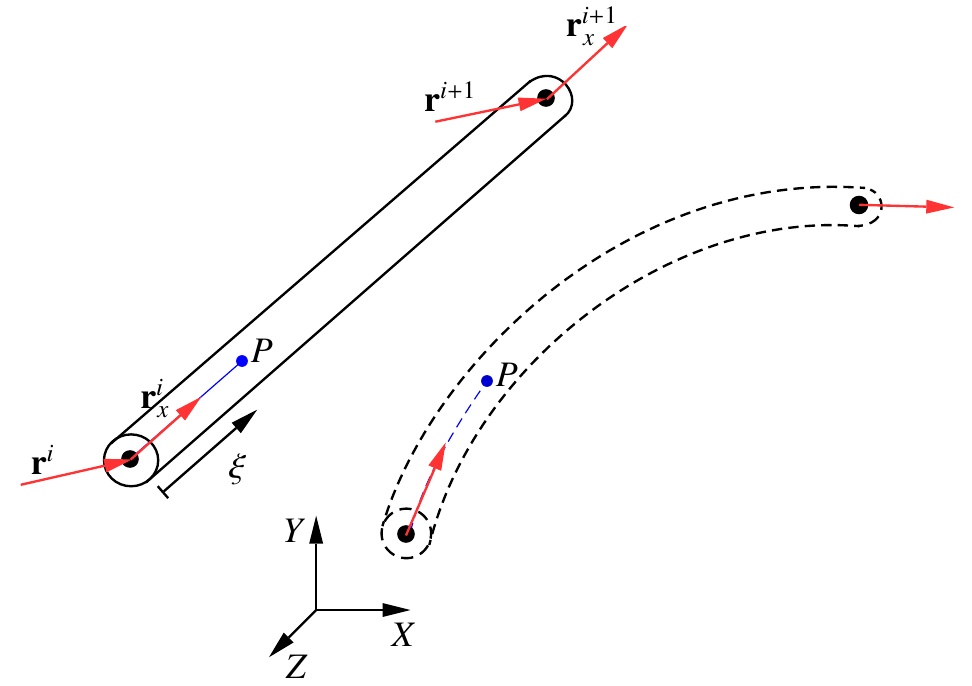
\includegraphics[width=.6\linewidth]{images/ANCF_1D.png}
	\end{center}
	\caption{ANCF cable element's schematic. Each node features a global position vector and a position vector gradient along the axis of the element (6DOF). Using shape functions and knowing $\xi$ one can interpolate the degrees of freedom to any point $P$ within the element. } \label{fig:ANCFCable}
\end{figure}


Knowing the axial and bending strains, one can define the internal loads of this element. 
The generalized element elastic forces are calculated as follows:
\begin{equation} \label{eq:ANCF_Beam_Qe}
\mathbf{Q}^i_{e}=\int\limits_{L}{\left[ EA \varepsilon_{x} ({\frac{{\partial \varepsilon }_{x}}{\partial \mathbf{q}}})^T+EI\kappa ({\frac{\partial \kappa}{\partial \mathbf{q}}})^T  \right]}\text{d}x,
\end{equation}
where $E$, $A$, and $I$ are the modulus of elasticity, the cross section area, and the area moment of inertia, respectively. The axial strain and curvature are defined as follows
\begin{equation*} \label{eq:ANCF_Beam_ex_k}
{{\varepsilon }_{x}}=\frac{1}{2}\left( \bm{r}_{x}^{\text{T}}\bm{r}_{x}^{{}}-1 \right) \text{  } \text{and} \text{  } \kappa \text{=}\frac{\left| {{\bm{r}}_{x}}\times {{\bm{r}}_{xx}} \right|}{{{\left| {{\bm{r}}_{x}} \right|}^{3}}},
\end{equation*}
where $\bm{r}^i_{x}=\bm{S}_x(\zeta) \bm{q}^i$ and $\bm{r}^i_{xx}=\bm{S}_{xx}(\zeta) \bm{q}^i$ terms involve differentiation of the shape function matrix $\bm S$.

Similarly, external applied forces, including those coming from the fluid system are interpolated to nodal coordinates and subsequently applied in the structural system via:
\begin{equation} \label{eq:ANCF_Beam_Qa}
Q^i_a = \bm S(x)^T \bm F.
\end{equation}

The generalized body forces including gravity force may be computed according to the standard finite element formulation as :

\begin{equation} \label{eq:ANCF_Beam_Qb}
Q^i_b = \int_{L} \rho_s A \bm S(x)^T \bm f_b,
\end{equation}
where $\rho_s$ and $A$ are the density and cross sectional area of the element, and $f_b$ is density of the body force. 


\subsection{ANCF Shell Element}\label{sec:2DElem}
The gradient-deficient ANCF shell element studied in \cite{Yamashita2015continuum} is used in the present work to simulate 2D flexible bodies. The nodal global position vector ($\mathbf{r}^{i}$) and global position vector transverse gradient ($\mathbf{r}_{z}^{i}=\frac{\partial {{\mathbf{r}}^{i}}}{\partial {{z}^{i}}}({{\xi}^{i}},{{\eta}^{i}})$) are chosen as the nodal degrees of freedom, as shown in Fig.~\ref{fig:ANCF_Shells}.

\begin{figure}[!t]
	\begin{center}
		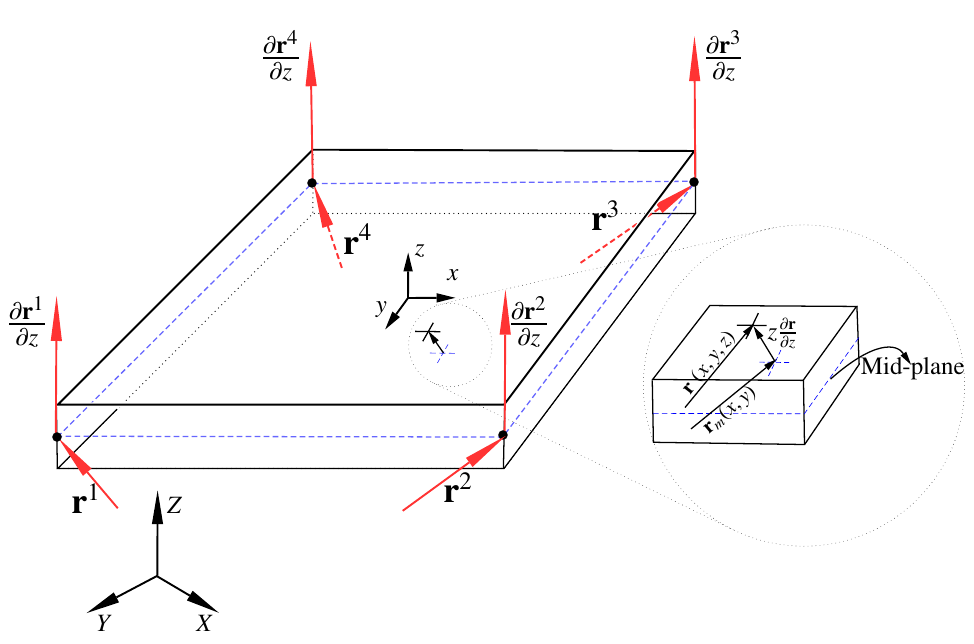
\includegraphics[width=.6\linewidth]{images/ANCF_2D.png}
	\end{center}
	\caption{ANCF shell element's schematic. Global position vector $\mathbf{r}^{j}$ and fiber's direction $\mathbf{r}_z^{j}=\frac{\partial {{\mathbf{r}}^{j}}}{\partial {{z}^{i}}}({{\xi}^{i}},{{\eta}^{j}})$ are the nodal coordinates of the $j^{th}$ node (6DOF). Using shape functions and knowing $\xi$ and $\eta$ one can interpolate the degrees of freedom to any point within the element. }\label{fig:ANCF_Shells}
\end{figure}

The positions and gradients on the mid-plane for any point inside the $i^{th}$ element can be interpolated from the positions and gradients of its nodes as follows
\begin{equation} \label{eq:ANCF_Shell_coordinates}
\mathbf{r}_{m}^{i}({{\xi}^{i}},{{\eta}^{i}})=\mathbf{S}_{m}^{i}({{\xi}^{i}},{{\eta}^{i}})\mathbf{e}_{p}^{i},\quad \frac{\partial {{\mathbf{r}}^{i}}}{\partial {{z}^{i}}}({{\xi}^{i}},{{\eta}^{i}})=\mathbf{S}_{m}^{i}({{\xi}^{i}},{{\eta}^{i}})\mathbf{e}_{g}^{i},
\end{equation}
where $\xi^i$ and $\eta^i$ refer to $i^{th}$ element's natural coordinates in the parametric space, $\mathbf{S}_{m}^{i}=\begin{bmatrix}
S_{1}^{i}\mathbf{I}& S_{2}^{i}\mathbf{I}& S_{3}^{i}\mathbf{I}&  S_{4}^{i}\mathbf{I}] \end{bmatrix}$ is a bilinear shape function matrix, $\mathbf{e}_{p}^{ij}={{\mathbf{r}}^{ij}}$ is the position vector of $j^{th}$ node of the element $i$, and $\mathbf{e}_{g}^{ij}={\partial {{\mathbf{r}}^{ij}}}/{\partial {{z}^{i}}}\;$ is the position vector gradient of node $j$ of element $i$, and $\textbf{I}$ is the $3\times 3$ identity matrix.
The bilinear shape functions of the ANCF shell element are given by the following expressions
\begin{equation*} \label{eq:ANCF_Shell_Shapefunctions}
\begin{split}
S_{1}^{i}=\frac{1}{4}(1-{{\xi }^{i}})(1-{{\eta }^{i}}), S_{2}^{i}=\frac{1}{4}(1+{{\xi }^{i}})(1-{{\eta }^{i}}),\\
S_{3}^{i}=\frac{1}{4}(1+{{\xi }^{i}})(1+{{\eta }^{i}}), S_{4}^{i}=\frac{1}{4}(1-{{\xi }^{i}})(1+{{\eta }^{i}}).
\end{split}
\end{equation*}
The position of an arbitrary point in the $i^{th}$ element may be described as
\begin{equation} \label{eq:ANCF_Shell_r}
{{\mathbf{r}}^{i}}({\xi}^i,{\eta}^i,{z}^i)={{\mathbf{S}}^{i}}({\xi}^i,{\eta}^i,{z}^i){{\mathbf{e}}^{i}},
\end{equation}
where ${{\mathbf{S}}^{i}}=[\begin{matrix} \mathbf{S}_{m}^{i} \,\,\, {{z}^{i}}\mathbf{S}_{m}^{i}\end{matrix}]_{3\times 24}$ is the combined shape function matrix, and $\quad {{\mathbf{e}}^{i}}= [{ \begin{matrix} {{(\mathbf{e}_{p}^{i})}^{T}} \,\,\, {{(\mathbf{e}_{g}^{i})}^{T}}\end{matrix}}]_{1\times 24}^T$ is the coordinates of the $i^{th}$ element grouped together. Eq.~\ref{eq:ANCF_Shell_r} allows for interpolating points along the element thickness by incorporating the element natural coordinate $z^i$.
The Green-Lagrange strain tensor, which is expressed as follows, 
\begin{equation} 
{{\mathbf{E}}^{i}}=\frac{1}{2}\left( {{\left( {{\mathbf{F}}^{i}} \right)}^{T}}{{\mathbf{F}}^{i}}-\mathbf{I} \right),
\label{eq:ANCF_E}
\end{equation}
is used to obtain the strains, where ${\mathbf{F}}^{i}$ is the deformation gradient matrix defined as the Jacobian of the current configuration over the reference configuration, which is expressed as 
\begin{equation} 
{{\mathbf{F}}^{i}}=\frac{\partial {{\mathbf{r}}^{i}}}{\partial {{\mathbf{X}}^{i}}}=\frac{\partial {{\mathbf{r}}^{i}}}{\partial {{\mathbf{x}}^{i}}}{{\left( \frac{\partial {{\mathbf{X}}^{i}}}{\partial {{\mathbf{x}}^{i}}} \right)}^{-1}}=  \bar {\bm J}^i  ({\bm J^i})^{-1}, \label{eq:ANCF_F}
\end{equation}
where $\dfrac{\partial {{\mathbf{r}}^{i}}}{\partial {{\mathbf{x}}^{i}}}=\bar {\bm J}^i$, and ${{ \dfrac{\partial {{\mathbf{X}}^{i}}}{\partial {{\mathbf{x}}^{i}}} }}= {\bm J^i}$. Incorporating \ref{eq:ANCF_F}, in \ref{eq:ANCF_E} results in
\begin{equation}
\bm{E}^i=({\bm{J}^i})^{-T} \tilde{\bm{E}}^i ({\bm{J}^i})^{-1},
\label{eq:ANCF_E2}
\end{equation}
where $\tilde{\bm{E}}^i$ the covariant strain tensor defined via:
\begin{equation}
{\tilde{\bm{E}}}^i=\frac{1}{2}\big( (\bar {\bm J}^i)^{T}  \bar {\bm J}^i -  (\bm J^i)^{T}  {\bm J}^i  \big)
\label{eq:ANCF_E_tilde}
\end{equation}
and can be re-expressed in a vector form as follows:
\begin{equation} \label{eq:equ7}
{{\bm{\tilde{\varepsilon} }}^{i}}={{\left[ \begin{matrix}
		\tilde{\varepsilon} _{xx}^{i} & \tilde{\varepsilon} _{yy}^{i} & \tilde{\gamma} _{xy}^{i} & \tilde{\varepsilon} _{zz}^{i} & \tilde{\gamma} _{xz}^{i} & \tilde{\gamma} _{yz}^{i} \\
		\end{matrix} \right]}^{T}}
\end{equation}
The engineering strain vector can be expressed in terms of the covariant strain vector as follows:
\begin{equation}
{{\bm{\varepsilon }}^{i}}=(\bm {T}^i)^{-T} {{\bm{\tilde{\varepsilon} }}^{i}},
\end{equation}
where the  engineering strain vector in the deformed configuration is defined via  
\begin{equation} \label{eq:equ8}
{{\bm{\varepsilon }}^{i}}={{\left[ \begin{matrix}
		\varepsilon _{xx}^{i} & \varepsilon _{yy}^{i} & \gamma _{xy}^{i} & \varepsilon _{zz}^{i} & \gamma _{xz}^{i} & \gamma _{yz}^{i} \\
		\end{matrix} \right]}^{T}}.
\end{equation}
Above, the constant transformation matrix (note that ${{\mathbf{J}}^{i}}$ only depends on the initial and reference configuration).
\begin{equation} \label{eq:equ10}\scriptsize
{{\mathbf{T}}^{i}}=\left[ \begin{matrix}
{{(J_{11}^{i})}^{2}} & {{(J_{12}^{i})}^{2}} & 2J_{11}^{i}J_{12}^{i} & {{(J_{13}^{i})}^{2}} & 2J_{11}^{i}J_{13}^{i} & 2J_{12}^{i}J_{13}^{i}  \\
{{(J_{21}^{i})}^{2}} & {{(J_{22}^{i})}^{2}} & 2J_{21}^{i}J_{22}^{i} & {{(J_{23}^{i})}^{2}} & 2J_{21}^{i}J_{23}^{i} & 2J_{22}^{i}J_{23}^{i}  \\
J_{11}^{i}J_{21}^{i} & J_{12}^{i}J_{22}^{i} & J_{11}^{i}J_{22}^{i}+J_{12}^{i}J_{21}^{i} & J_{13}^{i}J_{23}^{i} & J_{11}^{i}J_{23}^{i}+J_{13}^{i}J_{21}^{i} & J_{12}^{i}J_{23}^{i}+J_{13}^{i}J_{22}^{i}  \\
{{(J_{31}^{i})}^{2}} & {{(J_{32}^{i})}^{2}} & 2J_{31}^{i}J_{32}^{i} & {{(J_{33}^{i})}^{2}} & 2J_{31}^{i}J_{33}^{i} & 2J_{32}^{i}J_{33}^{i}  \\
J_{11}^{i}J_{31}^{i} & J_{12}^{i}J_{32}^{i} & J_{11}^{i}J_{32}^{i}+J_{12}^{i}J_{31}^{i} & J_{13}^{i}J_{33}^{i} & J_{11}^{i}J_{33}^{i}+J_{13}^{i}J_{31}^{i} & J_{12}^{i}J_{33}^{i}+J_{13}^{i}J_{32}^{i}  \\
J_{21}^{i}J_{31}^{i} & J_{22}^{i}J_{32}^{i} & J_{21}^{i}J_{32}^{i}+J_{22}^{i}J_{31}^{i} & J_{23}^{i}J_{33}^{i} & J_{21}^{i}J_{33}^{i}+J_{23}^{i}J_{31}^{i} & J_{22}^{i}J_{33}^{i}+J_{23}^{i}J_{32}^{i}  \\
\end{matrix} \right]\normalsize.
\end{equation}
The elastic internal forces are obtained by integration over the element volume using Gaussian quadrature as follows
\begin{equation} \label{eq:equ11}
\mathbf{Q}_{e}^{i}=\int\limits_{V_0^i}{\left( \frac{\partial {{\mathbf{\varepsilon }}^{i}}}{\partial {{\mathbf{e}}^{i}}} \right)^T} \sigma ^i \text{d}{{V}_{0}^i}\;,
\end{equation}
where $\mathbf{\sigma}^{i}$ is the vector of the second Piola-Kirchhoff stresses and $dV_i^0$ is the infinitesimal volume at the reference configuration of the element $i$.  

In order to alleviate the locking of the element, two modifications are performed on the strain's field of the element. The bilinear quadrilateral ANCF shell elements suffer from the in-plane shear/normal and transverse shear lockings, which can be eliminated using the ANS approach. Moreover, the use of position vector transverse gradient in this element causes thickness locking, which can be alleviated using the EAS approach. More details about the aforementioned approaches were provided in \cite{Yamashita2015continuum}.









\pagebreak